\documentclass[journal, a4paper]{IEEEtran}

% Essential Packages
\usepackage{graphicx}      % For inserting spectrograms and hardware diagrams
\usepackage{amsmath}       % For mathematical formulas (Welch's, 3-sigma)
\usepackage{hyperref}      % For clickable links to your GitHub repo
\usepackage{booktabs}      % For professional tables
\usepackage{cite}          % For citing literature (e.g., Berger's original work)
\usepackage{tabularx}
\usepackage{biblatex}
\addbibresource{bibliography.bib}

% Document Info
\title{Event-Related Alpha Desynchronization Brain Computer Interface Using Arduino UNO}
\author{Davide Masciola}


\begin{document}

\maketitle

\begin{abstract}
This report details the hardware architecture and digital signal processing pipeline of a real-time Brain-Computer Interface (BCI) designed to detect Event-Related Desynchronization (ERD) in the Alpha band (8–12 Hz) in the Occipital lobe. By utilizing an isolated electromechanical actuation loop and dynamic statistical thresholding, the system successfully generalizes across multiple human subjects with varying baseline neurophysiology, maintaining a robust Signal-to-Noise Ratio while eliminating PWM-induced electrical artifacts.
\end{abstract}

\begin{IEEEkeywords}
Brain-Computer Interface, Electroencephalography, Digital Signal Processing, Arduino, Alpha band.
\end{IEEEkeywords}

\section{Introduction}
\IEEEPARstart{T}{he} Alpha rhythm (8–12 Hz) is highly responsive to visual stimulus and attention. The attenuation of this rhythm, known as the Berger effect or Event-Related Desynchronization (ERD), is a well-known phenomenon in biomedical literature. It was first discovered by the German neurologist and psychiatrist Hans Berger in 1929 \cite{berger1929elektrenkephalogramm}; in 1934, Edgar Douglas Adrian and Bryan Matthews conducted further studies on the Berger effect, locating it in the Occipital lobe of the scalp \cite{adrian1934berger}; modern literature has described in detail the ERD phenomenon as a gain-control mechanism related to light adaptation \cite{pfurtscheller1999event}, \cite{kirschfeld2005physical}. The primary scope of this project is to capture the biological ERD and translate it into a reliable control mechanism for external electromechanical hardware, allowing the user to control a small servomotor by monitoring the Alpha band spectral power. The system combines compact design with audiovisual feedback to the user, by updating the board status during calibration and registration phases and printing guidance messages into the monitor. The whole architecture has been tested both with user+operator and user-only setup, being fully operational even without an external guidance. The further goal of the project was to guarantee maximum feasibility for its realization: the project has been successfully engineered with a total budget of roughly €100.
\begin{figure}[ht]
    \centering
    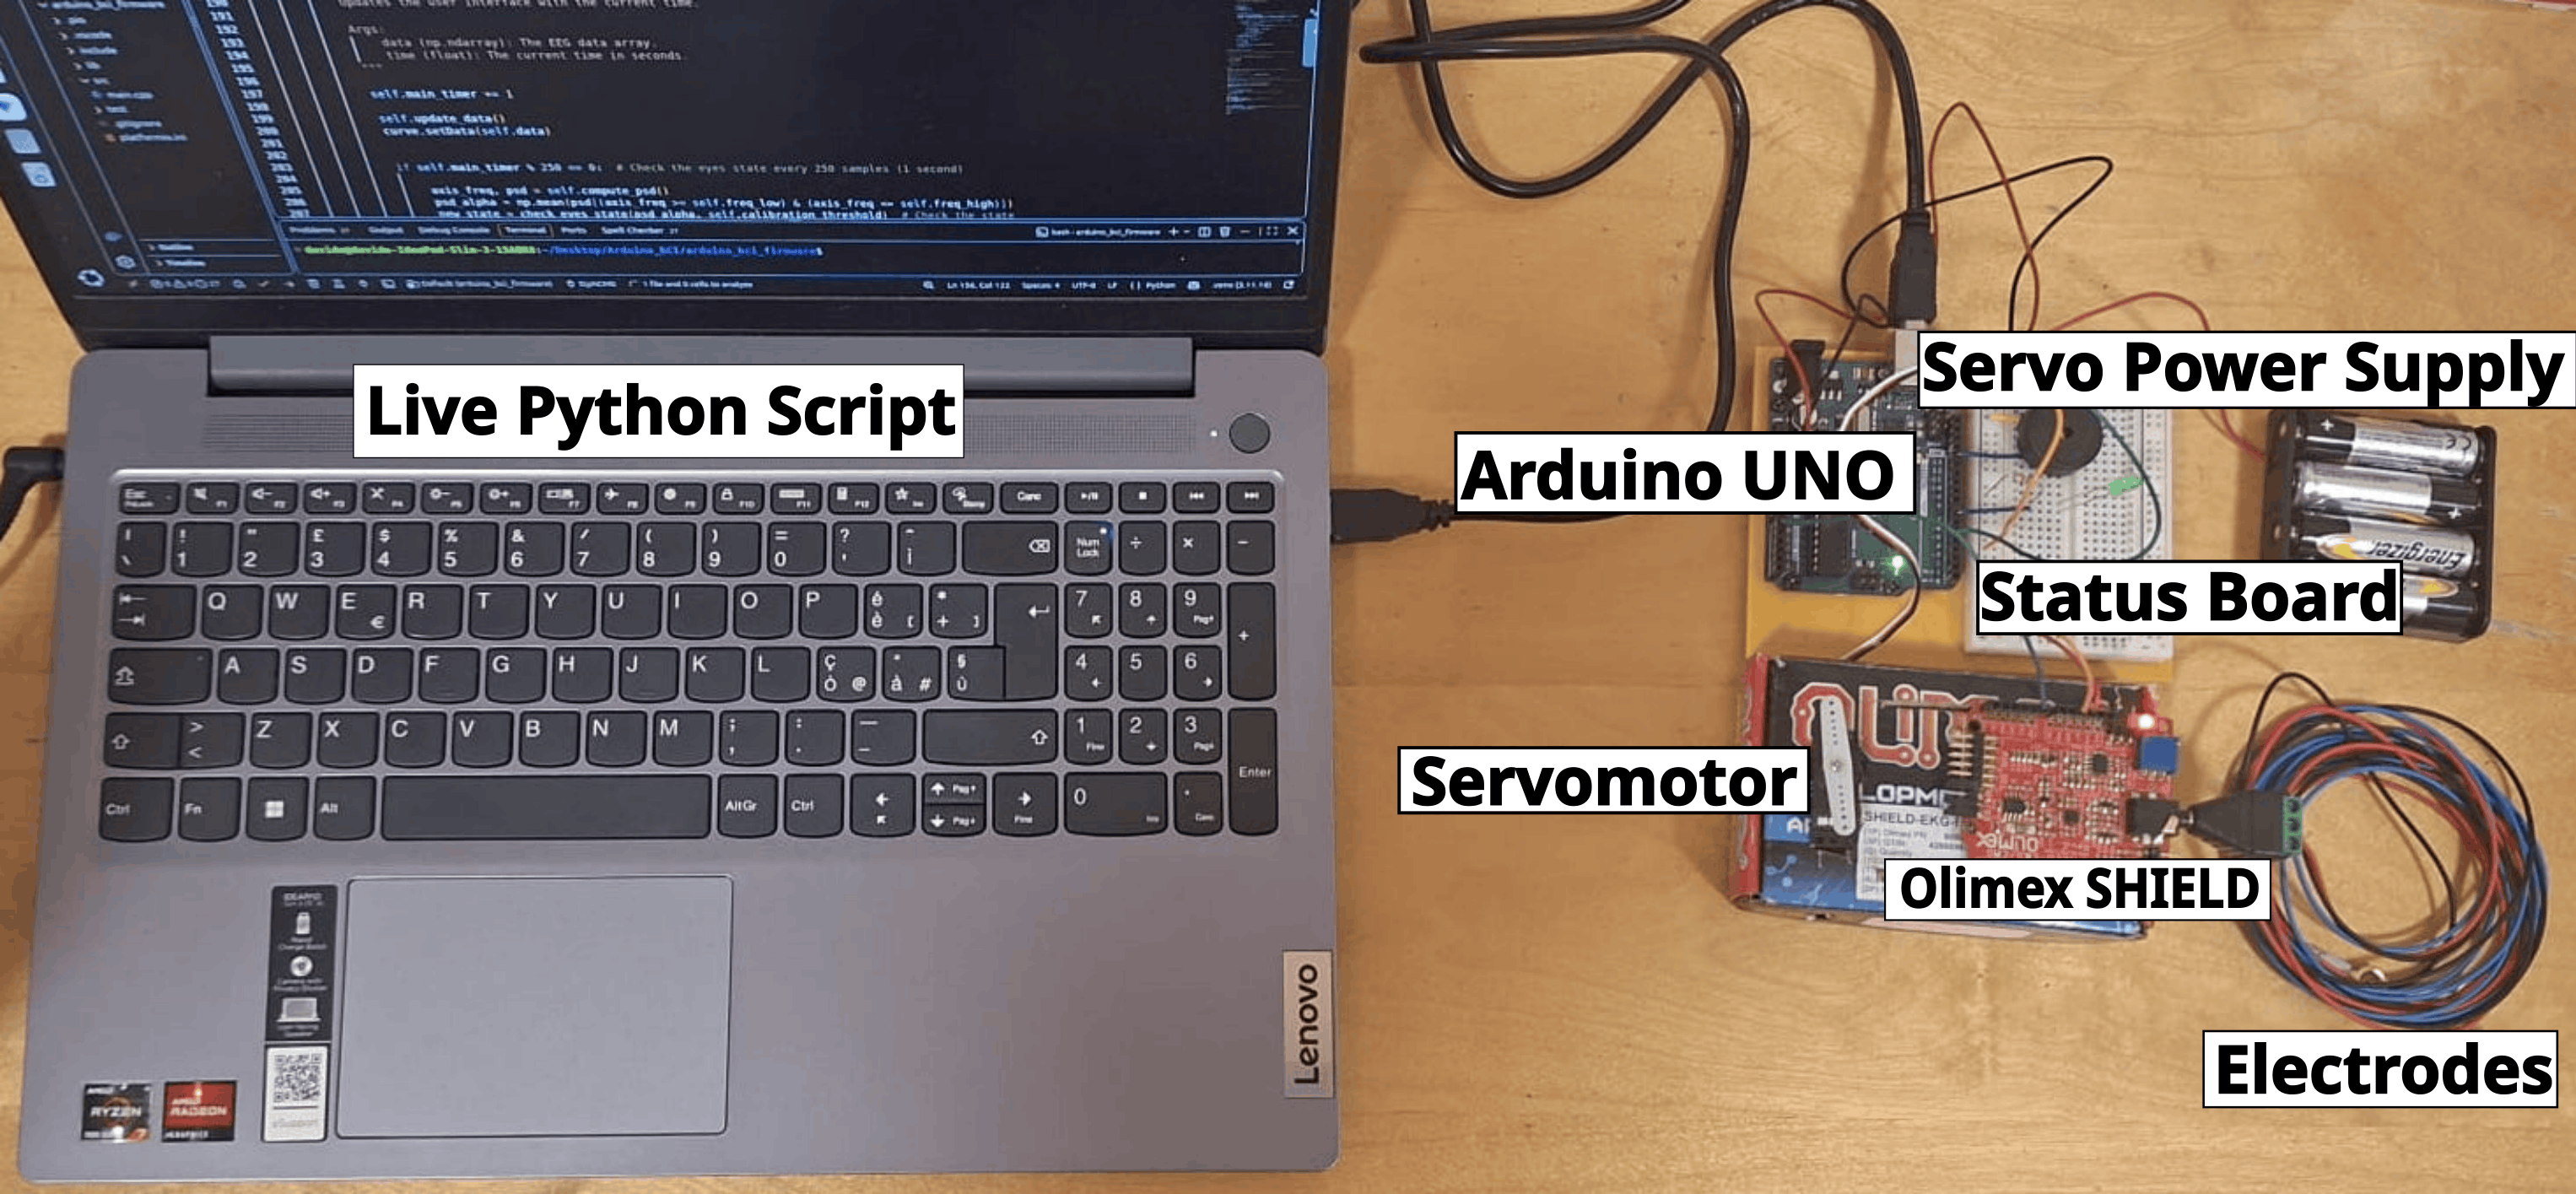
\includegraphics[width = 1\linewidth]{Images/Setup-1.png}
    \caption{Brain-Computer Interface setup.}
    \label{fig:placeholder}
\end{figure}

\section{Hardware Architecture \& Noise Mitigation}
To register the Occipital brain activity using electroencephalography (EEG), golden plated (Au) electrodes have been used. Au was preferred to Ag/AgCl due to its durability and ease of maintenance, providing a suitable resolution for the experiment and a low impedance combined with conductive paste and a skin cleanser. The three electrodes are placed respectively on Oz (Channel +), Mastoid (Channel -), and Fz (Ground).
\begin{figure}[ht]
    \centering
    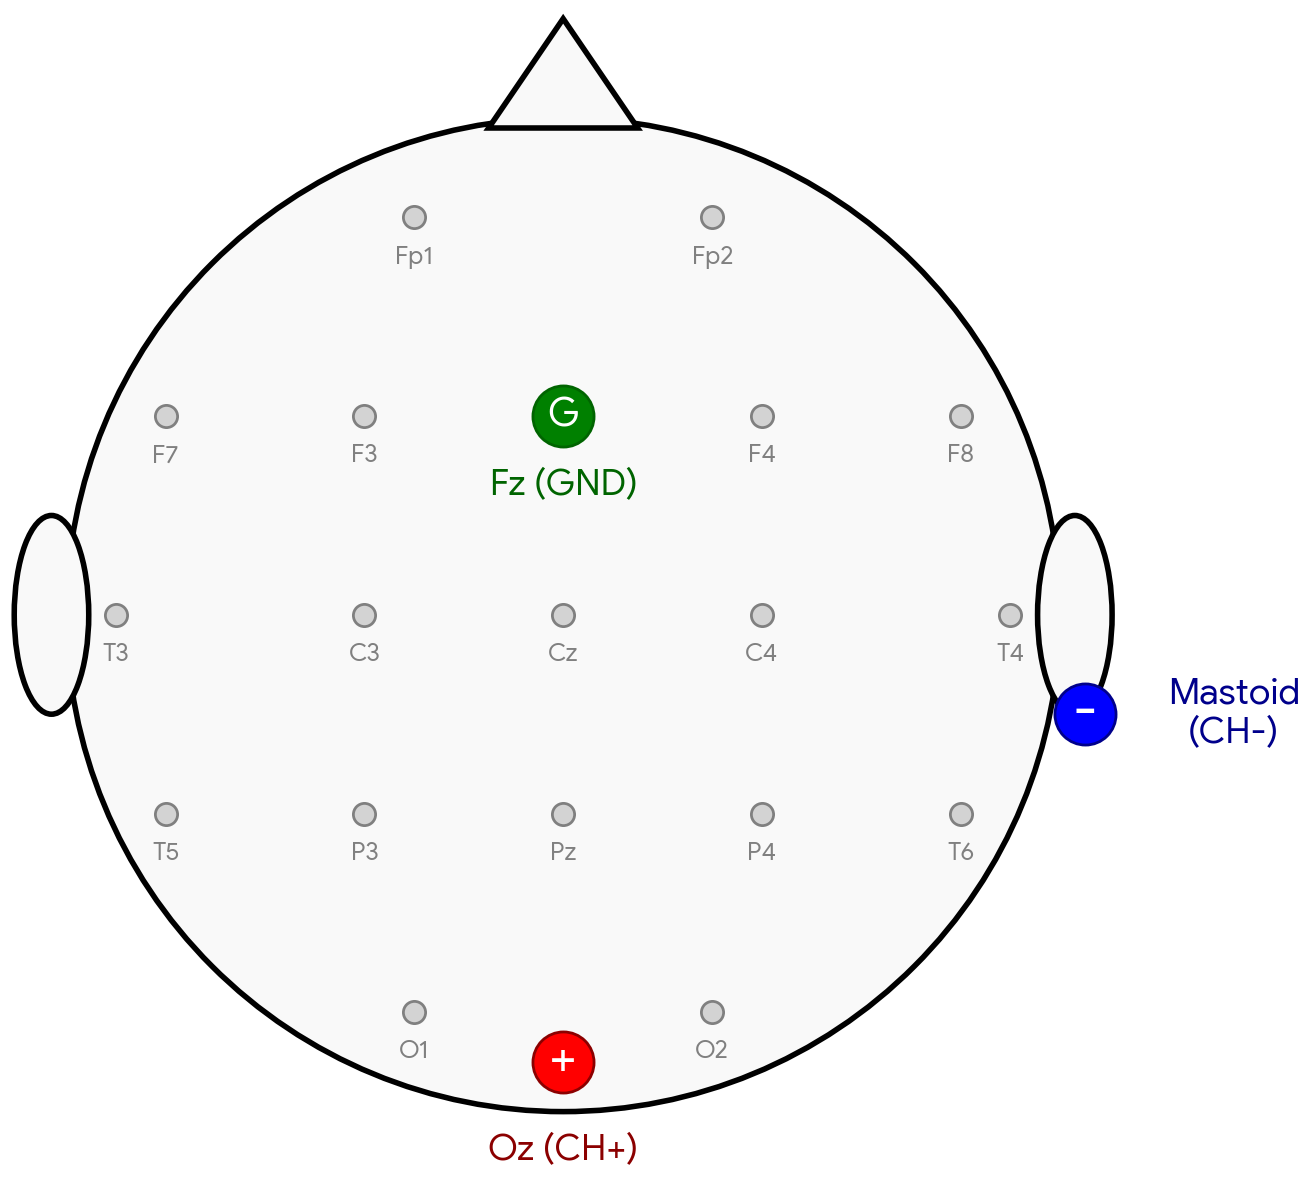
\includegraphics[width=0.5\linewidth]{Images/Electrode Positioning.png}
    \caption{Electrodes placement.}
    \label{electrodes}
\end{figure}

A significant challenge in closed-loop EEG systems is the registration of the signal and its amplification. To mitigate the noise of the EEG system, KONIX EEG Paste was applied to minimize impedance and secure the electrodes on the scalp. To amplify the signal from the usual $\sim \mu V$ range to the correct amplitude for the A/D converter, the electrodes are connected to the OLIMEX SHIELD EKG-EMG biosignal amplifier, with the following pipeline.
\begin{equation*}
    \text{Instr. Amp}\rightarrow\text{Besselworth 40Hz Lowpass Filter}\rightarrow\text{OAmp}
\end{equation*}
The OAmp was left with the default ($\sim$80) gain, bringing the $G_\text{total} = 10*80*3.46 = 2848$.

The SHIELD is powered by the Arduino board at 5 V and sends the digital data to the A0 port of the Arduino. The board also powers a green LED and a piezo speaker to provide visual and audio feedback to the user about the state of the machine. The EEG data is then sent in a 4 byte packet containing a start and a end sequence and the 10 bit signal in between. This configuration allows the computer program to correctly recognize the single data packet and synchronize with the board. A USB cable both powers the system and allows communication between the board and the computer. 

The servomotor is powered separately with a 6 V battery to avoid PWM noise in the SHIELD: if the squared wave sent from Arduino to power the servo is connected in parallel with the board, a small percentage of the signal enteres the amplification pipeline, producing huge bumps that completely disrupt the signal.

\section{BCI Pipeline}
The entire BCI pipeline is shown below.
\begin{figure}[ht]
    \centering
    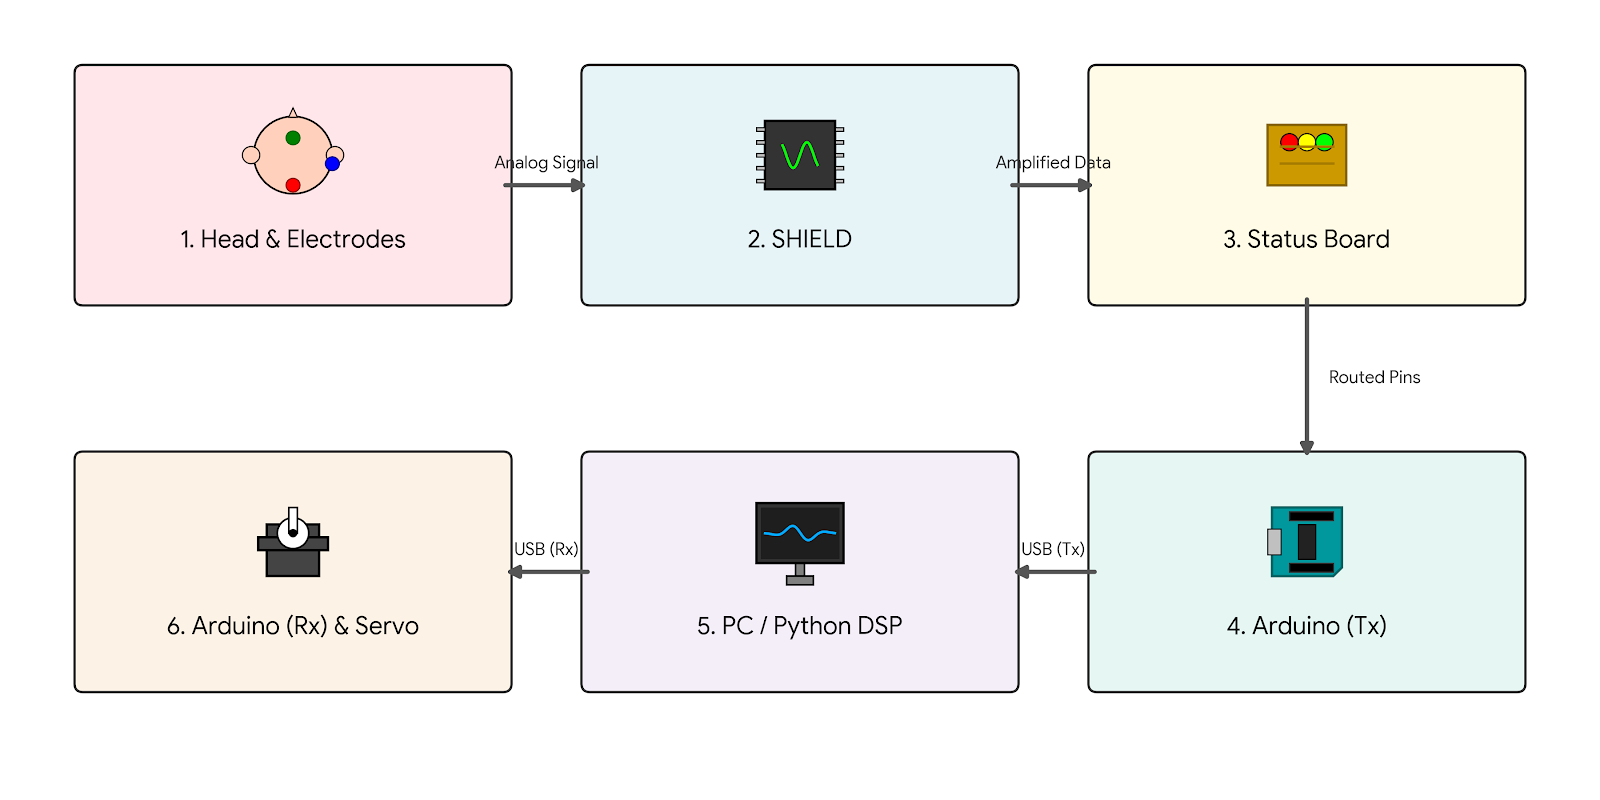
\includegraphics[width=1\linewidth]{Images/Processing Pipeline.png}
    \caption{The BCI Pipeline.}
    \label{fig:placeholder}
\end{figure}

\begin{enumerate}
    \item The electrodes placed on the head record the biopotential. Ground common mode signal is mitigated and the Mastoid CH- accounts for muscle artifacts.
    \item The SHIELD amplifies and filters the analog signal.
    \item The board shows the BCI status. A green led is on during all the data acquisition procedure.
    \item The Arduino UNO converts the data to a digital 4-byte packet. Data is converted based on the 5\,V scale based on the relation
    \begin{equation*}
        \text{Data}=\frac{S}{V}*2^{10}
    \end{equation*}
    Where \textit{S} is the analog signal and \textit{V} is the power line of the board (5\,V).
    \item The pc reads the packet and analyzes the data. The processing is described in Chapter \ref{processing}.
    \item The pc feedback is sent back to the Arduino as a ASCII conversion of a char value, which is evaluated to correctly actuate the servo.
\end{enumerate}

\section{Signal Processing}\label{processing}
The continuous data stream is sampled at 250\,Hz to provide a solid and precise signal. The digital signal processing is managed by the python live script. The script is responsible for calibration, synchronization of the data collection process, data plotting, data filtering, spectral power estimation and response evaluation, and data storage. The choice of the coding language is justified by the useful libraries for signal processing and the ease of use for running live scripts.

\subsection{Data collection}
The script is set to accept data from a specified serial port, the packet received is then checked with the start and end sequence and the information content is then stored in a numerical array. The length of the array has been set to 5 minutes of registration ($5*60*Fs = 75*10^{3}$ samples). This specific length allows the data to be collected for a sufficient and adjustable time window without the risk of RAM overflow. After exactly five minutes from the start of the experiment, the array is stored in a CSV file to allow for offline analysis, the script keeps running until stopped by the user.

\subsection{Bandpass Filtering}
A 4th-order Butterworth bandpass filter isolates the 8--12\,Hz frequency band. Choosing to use Infinite Impulse Response (IIR) Filters allows low-latency filtering due to the low order, and a good mitigation of cutoff frequencies with a negligible distorsion (both ripple and nonlinear phase) for the specific application.

\subsection{Spectral Estimation and Windowing}
Power Spectral Density (PSD) is calculated using Welch's method. The estimation is made on a 4 second window during calibration phase, and is then executed on every new second (250 samples) of registration. Such time windows provide robust threshold estimation and dynamic power evaluation to correctly describe the power increase/decrease.

\section{Dynamic Calibration \& Results}
Because biological signals exhibit immense physiological variance across individuals, static amplitude thresholds frequently fail. The system provides high adaptability to different users by implementing an initial phase of calibration. The process is divided into 4 steps:
\begin{enumerate}
    \item 5 second registration in active (eyes open) state. Estimation of low Alpha-band mean power $\text{m}_{\text{active}}$.
    \item 5 second registration in rest (eyes closed) state. Estimation of high Alpha-band mean power $\text{m}_{\text{rest}}$.
    \item Evaluation of spectral power levels. The script returns an error if the high level is below the lower level and prints a warning if the high level is less than 1.5 times the low level (which might be caused by bad electrode connection).
    \item Estimation of threshold \textit{T}.
\end{enumerate}

\subsection{Artifact Rejection \& Outliers Robustness}
To avoid including any movement that the user might do during the change from  active (eyes open) and the rest (eyes closed) state, a transition time is added between the calibration steps. For additional mitigation of accidental artifacts, the Spectral Power estimation is calculated over a 4 second window extracted from the 5 second window registered, so the first second of the calibration procedure is automatically rejected.  

To mitigate servo twitching during the experiment---a behavior shown in early tests that was related to false positives/negatives and only lasted one window frame---the state evaluation system compares the new power window $\text{P}_{\text{new}}$ to the last two windows evaluated $\text{P}_{\text{current}}$ and $\text{P}_{\text{past}}$. The algorithm logic is:
\begin{itemize}
    \item if $\text{P}_{\text{new}}$ == $\text{P}_{\text{current}}$ AND $\text{P}_{\text{new}}$ $\ne$ $\text{P}_{\text{past}}$: the servo changes its state.
    \item else: the servo does not change its state.
\end{itemize}
Although this method introduces 1 second of latency to the actuation of the mechanism, it provides a much more precise response, actuating correctly in response to a change of state.
\subsection{Statistical Thresholding}
The transition threshold $T$ is defined dynamically using a 3-sigma confidence interval based on the user's resting Alpha power:
\begin{equation*}
T = m_{\text{rest}} + 3*s_{\text{rest}}
\end{equation*}
Where $\text{m}_{\text{rest}}$ and $\text{s}_{\text{rest}}$ are the sample's mean and standard deviation.

This confidence interval of roughly 99\% provides precise response to the user's input, as shown in the test trials.


\subsection{Offline Validation}
Offline MATLAB analysis of continuous Alpha power revealed significant physiological variance among the tested subjects. Subjects demonstrating high Event-Related Desynchronization achieved a linear Signal-to-Noise Ratio (SNR) exceeding 4.0 (with a registered maximum of 6.69 dB). However, the system also successfully adapted to subjects with heavily attenuated Alpha responses (SNR 3.19/4.98 dB). A static threshold calibrated for high-amplitude subjects would have resulted in a false-negative failure rate for low-amplitude users. The implementation of the dynamic 3-sigma statistical threshold successfully mitigated this physiological variance, ensuring robust electromechanical actuation across all subjects. 

To underline the adaptability of the system to physiological variance, the two most significant samples of high and low ERD are shown in Table \ref{tab:snr_results} and Figures \ref{subject1}, \ref{subject2}. Specifically, Subject1 shows an exceptional example of ERD, with a visible difference between the two states, while Subject2 presents a mild, yet noticeable difference. It should also be noted that some of the subjects presented anomalous spikes that were recorded in the low-power region, but most of these outliers were successfully tackled by the two-windows delay implemented in the algorithm.

\begin{table}[ht]
\centering
\caption{Signal-to-Noise Ratio (SNR) Analysis of Alpha-Band Event-Related Desynchronization}
\label{tab:snr_results}
\setlength{\tabcolsep}{3pt} % Compresses horizontal padding between columns
\begin{tabular}{@{}lcccc@{}}
\toprule
\textbf{Subject} & \textbf{Baseline (Opened)} & \textbf{Active (Closed)} & \textbf{SNR (Linear)} & \textbf{SNR (dB)} \\ \midrule
Subject1          & 0.3261                     & 1.5218                   & 4.67                  & 6.69              \\ 
Subject2         & 0.2042                     & 0.6426                   & 3.15                  & 4.98              \\\bottomrule
\end{tabular}
\end{table}
\begin{figure}[ht]
    \centering
    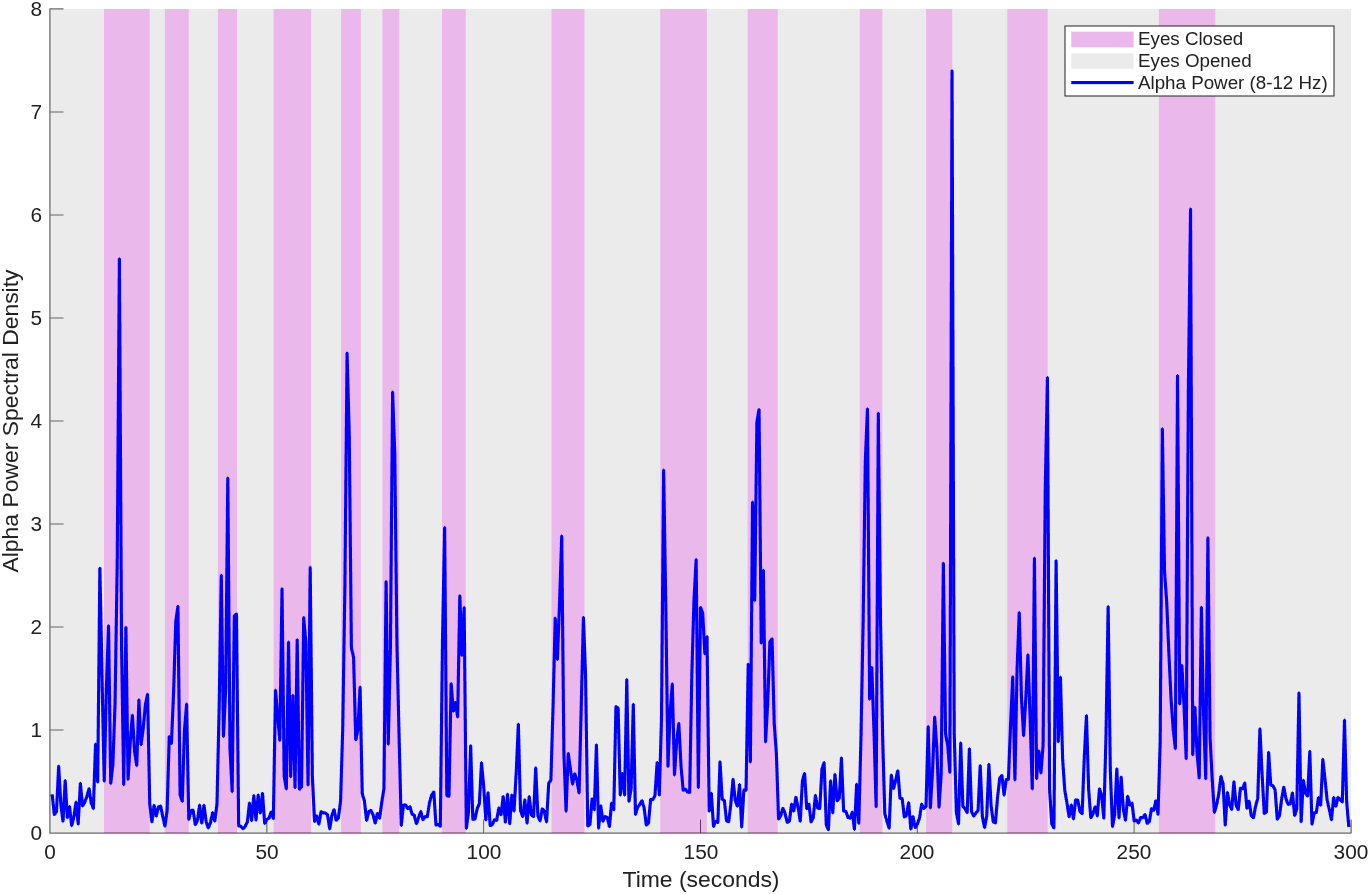
\includegraphics[width=0.8\linewidth]{Images/SubjectHighSNR.png}
    \caption{Subject1 (6.69 dB SNR)}
    \label{subject1}
\end{figure}

\begin{figure}[ht]
    \centering
    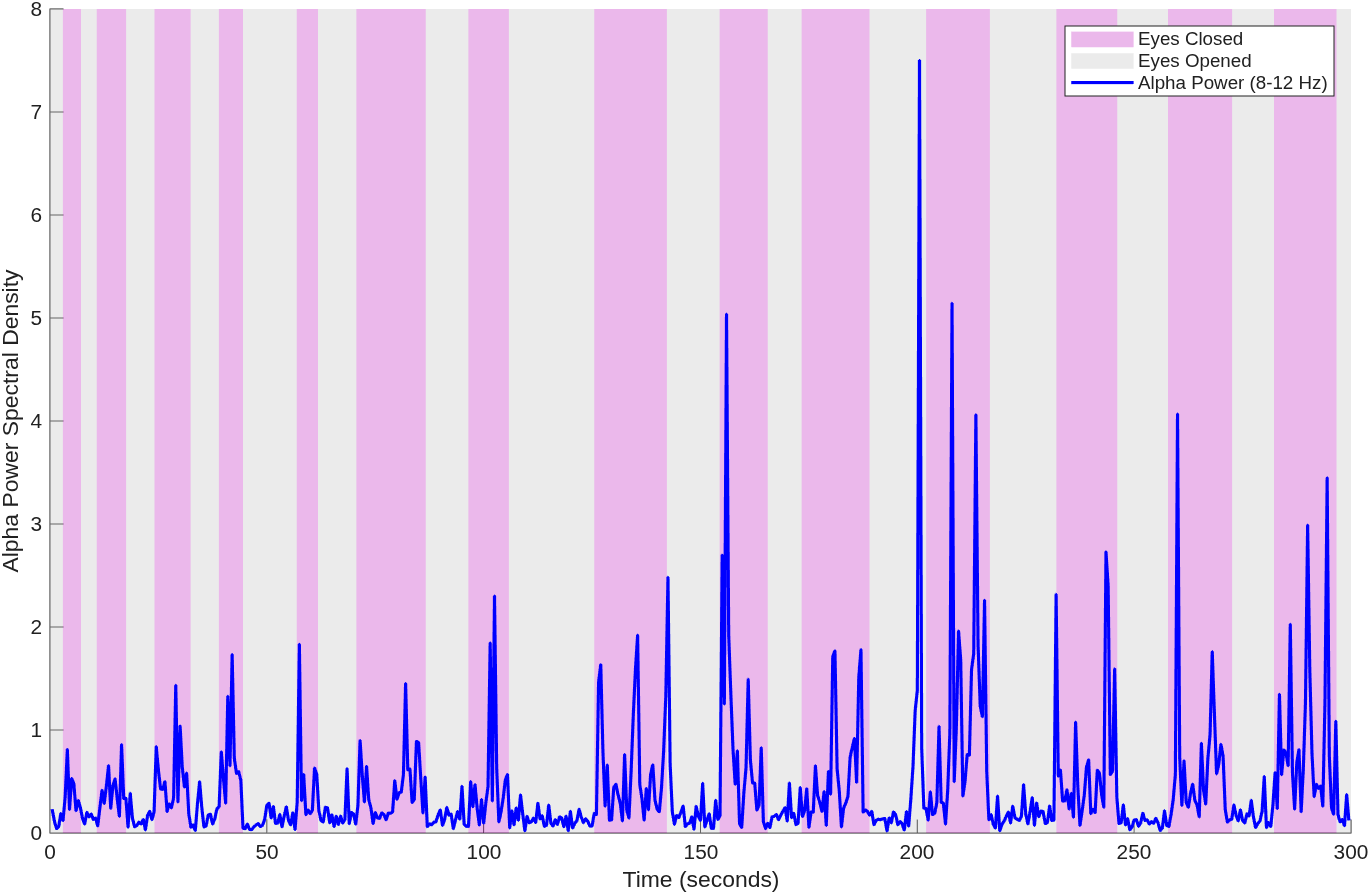
\includegraphics[width=0.8\linewidth]{Images/SubjectLowSNR.png}
    \caption{Subject2 (4.98 dB SNR)}
    \label{subject2}
\end{figure}

The cases show a correct registration of Alpha-band spikes during resting state (colored windows). The dynamic threshold allows the servo to be controlled adapting to the subject's physiological PSD.


\section{Discussion \& Lessons Learned}
Hardware-software co-design is critical in biomedical engineering. Even with correct electrode placement, DSP algorithms cannot work properly with a physically compromised signal. For this reason, securing the hardware grounding was a mandatory prerequisite for software filters and algorithms to function. Furthermore, the necessity of adaptive baselining was proven: static thresholds are unviable for general-purpose BCIs, providing good suitability for the majority of subjects.

\section{Conclusion}
By combining strict hardware isolation with an adaptive, statistically grounded software threshold, this system provides a robust framework for real-time BCI control, generalizable across multiple users without manual recalibration.

\printbibliography

\end{document}